\begin{center}
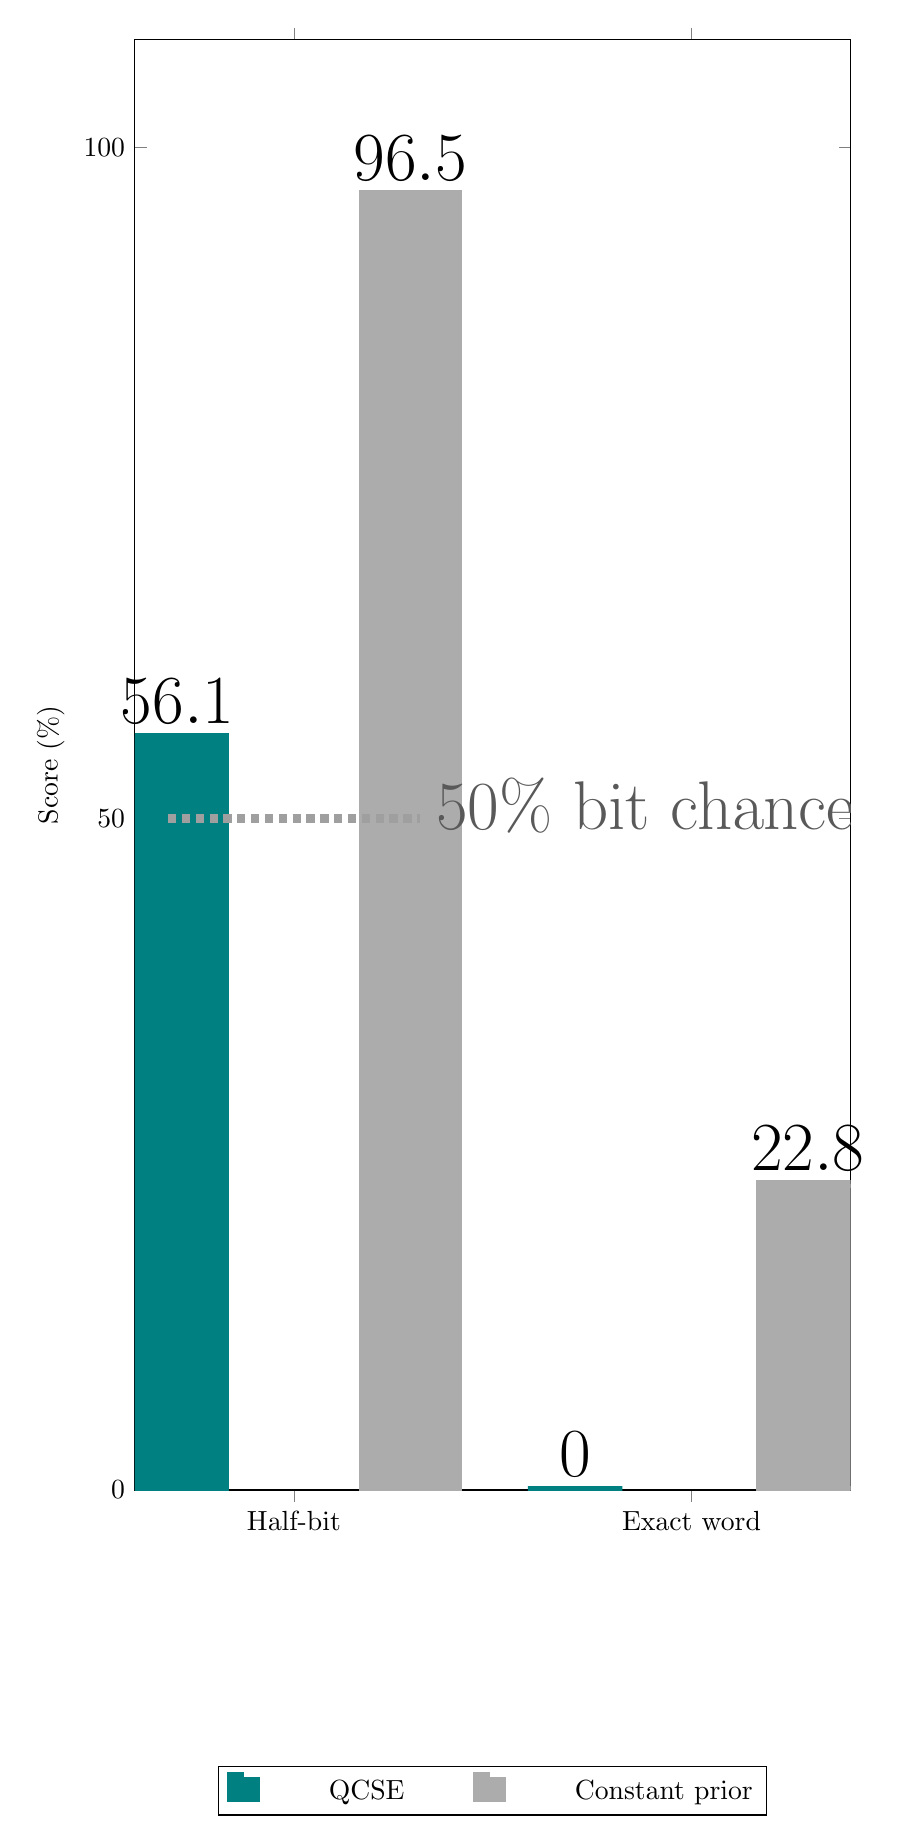
\begin{tikzpicture}
\begin{axis}[
  ybar,
  width=0.88\linewidth,
  height=20cm,
  xmin=0.3,xmax=5.7,
  ymin=0,ymax=108,
  ylabel={Score (\%)},
  xtick={1.5,4.5},
  xticklabels={Half-bit,Exact word},
  ytick={0,50,100},
  bar width=1.2cm,
  enlarge x limits=false,
  legend style={at={(0.5,-0.19)},anchor=north,legend columns=2,column sep=0.8cm},
  every axis plot/.append style={line width=3pt},
  nodes near coords={\pgfmathprintnumber[fixed,precision=1]\pgfplotspointmeta},
  nodes near coords style={font=\fontsize{24}{28}\selectfont,anchor=south}
]
  \addplot[fill=teal,draw=teal] coordinates {(1,56.1) (4,0)};
  \addlegendentry{QCSE}
  \addplot[fill=gray!65,draw=gray!65] coordinates {(2,96.5) (5,22.8)};
  \addlegendentry{Constant prior}
  \draw[gray!75,densely dashed,line width=3pt] (axis cs:0.55,50) -- (axis cs:2.45,50);
  \node[font=\fontsize{24}{28}\selectfont,anchor=west,text=gray!70!black] at (axis cs:2.5,51) {50\% bit chance};
\end{axis}
\end{tikzpicture}
\end{center}
\par\smallskip
\begin{minipage}{\linewidth}
\RaggedRight\fontsize{24}{29}\selectfont
57 targets; 96.5\% is not word recovery.
\end{minipage}
